\documentclass[10pt,a4paper]{article}
\usepackage[utf8]{inputenc}
\usepackage[french]{babel}
\usepackage[T1]{fontenc}
\usepackage{amsmath}
\usepackage{amsthm}
\usepackage{amsfonts}
\usepackage{amssymb}
\usepackage{graphicx}
\usepackage{mathrsfs}
\usepackage{url}
\usepackage[french,onelanguage,ruled,lined,linesnumbered]{algorithm2e}
\SetKw{And}{et}
\SetKw{From}{allant de}
\author{\textsc{TRAN Quoc Nhat Han} \& \textsc{Adrien WARTELLE}}
\title{Rapport de projet OS01}
\date{\today}
\begin{document}
\maketitle
\renewcommand{\contentsname}{Sommaire}
\tableofcontents
\clearpage

\section{Calcul d'un arbre de longueur minimale}

Basé sur le principe de Prim, nous proposons 3 algorithmes que nous appellons respectivement \emph{Naive}, \emph{Improved} et \emph{Best}.

Pour la consistence entre le code et le rapport, nous conservons les noms de variables (qui sont anglais dans le code actuel).

\subsection{Structures de données principales}

\subsubsection{\texttt{Point}}

Un point est défini un couple de réels positifs $(x, y)$ majorés par \texttt{maxX} et \texttt{maxY} respectivement.

De même, nous définissons le racine (\texttt{root}) avec les coordonnées $(0, 0)$.

Les points entrées sont lus et enregistrés au tableau \texttt{inputPoints}. Le racine est mis par défaut à \texttt{inputPoints[0]}.

Désormais, tous les autres variables dans le programme utiliseront la position du point dans \texttt{inputPoints} au lieu de recopier les valeurs de coordonnées, afin d'économiser la mémoire.

\subsubsection{\texttt{dist2} : Table de distances}

En général, dans 3 approches, nous calculons leurs distances et stockons en avance dans un tableau \texttt{dist2} afin d'éviter de recalculer les distances entre les points à chaque itération.

\texttt{dist2[i][j]} est la distance \emph{en carré} entre l'i-ième point et l'j-ième point. Notons que l'opération racine est couteuse et $0<x<y \Leftrightarrow x^2 < y^2$. Par conséquence, comparer deux distances de couples $(i_1, j_1)$ et $(i_2, j_2)$ revient à comparaison de \texttt{dist2[i1][j1]} et \texttt{dist2[i2][j2]}.

\subsubsection{\texttt{network} : L'arbre à construire}

Cet arbre consite d'un registre des points ajoutés (\texttt{vertex}) accompagné avec le compteur \texttt{n}, d'un registre des branches créés (\texttt{edge}) accompagné avec le compteur \texttt{m}, et un compteur de longueur total (\texttt{totalLength}).

\subsection{Algorithmes implémentés}

$N$ dénote le nombre de points entrées.

Cet arbre devra contient exactement $N$ branche. Chaque algorithme propose une approche différente à la recherce de nouvelle minimale branche.

\subsubsection{Naive}

L'algorithme \emph{Naive} cherche franchement, à chaque itération, dans le tableau \texttt{dist2} le distance $(i,j)$ le plus court tel que $i \in network$ et $j \not \in network$, puis il ajoute $j$ et sa liaison $(i,j)$ au \texttt{network}.

La détection de l'attache à l'arbre est faite par le tableau booléan \texttt{inTree} : \texttt{inTree[i]} vaut \texttt{true} si l'i-ième point appartient à \texttt{network}, et sinon \texttt{false}.

\begin{algorithm}[H]
    \caption{Algorithme Naive}
    \tcp{L'ajout de la branche i-ième}
    \For{$i$ \From $1$ \KwTo $N$}{
        \tcp{Initialisation}
        $newEdgeStart \leftarrow 0$\;
        $newEdgeEnd \leftarrow -1$\;
        $dist2Min \leftarrow maxX^2 + maxY^2$\;
        \For{$j$ \From $0$ \KwTo $N$}{
            \tcp{Recherche d'un point de début}
            \If{$j \in network$}{
                \tcp{Recherche d'un point de fin}
                \For{$k$ \From $0$ \KwTo $N$}{
                    \If{$k \neq j$ \And $k \not \in network$}{
                        \If{$dist2[j][k] < dist2Min$}{
                            $newEdgeStart \leftarrow j$\;
                            $newEdgeEnd \leftarrow k$\;
                            $dist2Min = dist2[j][k]$\;
                        }
                    }
                }
            }
            Ajouter $newEdgeEnd$ au $network$\;
            Ajouter la branche $(newEdgeStart, newEdgeEnd)$ au $network$\;
        }
    }
\end{algorithm}

Comme nous avons 3 boucles embriquées parcourant de $1$ ou $0$ à $N$, la complexité d'algorithm est donc $O(N^3)$.

\subsubsection{Improved}

Amélioré de \emph{Naive}, \emph{Improved} utilise le tableau \texttt{orderedPoints} pour stocker les points entrées dans l'ordre d'ajoute au \texttt{network}. C'est-à-dire, si \texttt{network} possède déjà $n$ points, le point \texttt{orderedPoints[i]}-ième est ajouté au \texttt{network} ($i=\overline{0, n-1}$), la reste est dehors.

\begin{algorithm}[H]
    \caption{Algorithme Improved}
    \tcp{L'ajout de la branche i-ième}
    \For{$i$ \From $1$ \KwTo $N$}{
        \tcp{Initialisation}
        $newEdgeStart \leftarrow 0$\;
        $newEdgeEnd \leftarrow -1$\;
        $dist2Min \leftarrow maxX^2 + maxY^2$\;
        \For{$j$ \From $0$ \KwTo $network.n - 1$}{
            \tcp{Grace à la définition de \texttt{orderedPoints}}
            \tcp{Recherche d'un point de début est réduit à}
            \tcp{\texttt{orderedPoints[0]} jusqu'au}
            \tcp{\texttt{orderedPoints[network.n - 1]}}
            $inNode \leftarrow orderedPoints[j]$\;
            \If{$j \in network$}{
                \tcp{Recherche d'un point de fin est réduit à}
                \tcp{\texttt{orderedPoints[network.n]} jusqu'au}
                \tcp{\texttt{orderedPoints[N]}}
                \For{$k$ \From $network.n$ \KwTo $N$}{
                    $outNode \leftarrow orderedPoints[k]$\;
                    \If{$dist2[inNode][outNode] < dist2Min$}{
                        $newEdgeStart \leftarrow j$\;
                        $newEdgeEnd \leftarrow k$\;
                        $dist2Min = dist2[inNode][outNode]$\;
                    }
                }
            }
            Ajouter $orderedPoints[newEdgeEnd]$ au $network$\;
            Ajouter $orderedPoints[newEdgeEnd]$ au fin des points intérieurs de $orderedPoints$\;
            Ajouter la branche $(orderedPoints[newEdgeStart], orderedPoints[newEdgeEnd])$ au $network$\;
        }
    }
\end{algorithm}

Bien que le nombre d'éléments à parcourir de 2 boucles intérieuses a diminué 2 fois, la complexité de cet algorithme reste $O(N^3)$.

\subsubsection{Best}

La version meilleure utilise le tableau \texttt{nearestNetworkNeighbor} indiquant le voisin le plus proche du point j-ième. Le tableau est mis à jour de manière sélective pendant chaque itération, grâce à la variable \texttt{newestNode}, qui stocke le point récemment ajouté.

\begin{algorithm}[H]
    \caption{Algorithme Best}
    \tcp{L'ajout de la branche i-ième}
    \For{$i$ \From $1$ \KwTo $N$}{
        \tcp{Initialisation}
        $newEdgeStart \leftarrow 0$\;
        $newEdgeEnd \leftarrow -1$\;
        $dist2Min \leftarrow maxX^2 + maxY^2$\;
        \For{$j$ \From $0$ \KwTo $N$}{
            \tcp{Recherche d'un point de fin}
            \If{$j \not \in network$}{
                \tcp{Mettre à jour le voisin le plus proche de j}
                \tcp{en comparant le newestNode et nearestNetworkNeighbor[j]}
                \If{dist2[newestNode][j] < dist2[nearestNetworkNeighbor[j]][j]}{
                    nearestNetworkNeighbor[j] = newestNode\;
                }
                \tcp{Chercher la branche la plus courte}
                \If{dist2[nearestNetworkNeighbor[j]][j] < dist2Min}{
                    dist2Min = dist2[nearestNetworkNeighbor[j]][j]\;
                    newEdgeStart = nearestNetworkNeighbor[j]\;
                    newEdgeEnd = j\;
                }
            }
            Ajouter $newEdgeEnd$ au $network$\;
            Ajouter la branche $(newEdgeStart, newEdgeEnd)$ au $network$\;
        }
    }
\end{algorithm}

A l'aide de \texttt{newestNode} et \texttt{nearestNetworkNeighbor}, nous économisons un boucle, résultant la complexité de l'ordre $O(N^2)$, qui est le meilleur possible selon les calculs démontrés de Prim.

\subsection{Exécution, mesure et visualisation}

En utilisant \emph{MersenneTwister.h}, nous générons des jeux de données de tailles différentes: $N=5,10,100,200,500,1000,10000$.

Spec de l'ordinateur à tester: Lenovo Y520, Intel(R) Core(TM) i7-7700HQ, CPU@2.8GHz(8CPUs), RAM 8192MB.

\begin{table}[!ht]
    \begin{center}
        \begin{tabular}{ |c|c|c|c| }
            \hline
            N		&		Naive		    &		Improved		&		Best\\
            \hline
            5		&		0,014587		&		0,003282		&		0,013128\\
            \hline
            10		&		0,026986		&		0,004011		&		0,010211\\
            \hline
            100		&		2,920300		&		0,233755		&		0,050324\\
            \hline
            200		&		5,043060		&		1,77413		    &		0,163373\\
            \hline
            500		&		161,429000		&		28,331		    &		3,527840\\
            \hline
            1000	&		1169,760000		&		265,508000		&		4,60399\\
            \hline
            10000	&		> 60000   		&		>60000	 		&		402,536000\\
            \hline
        \end{tabular}
    \end{center}   
    \caption{Table de temps d'exécution (ms)}     
\end{table}

\begin{figure}[!ht]
    \centering
    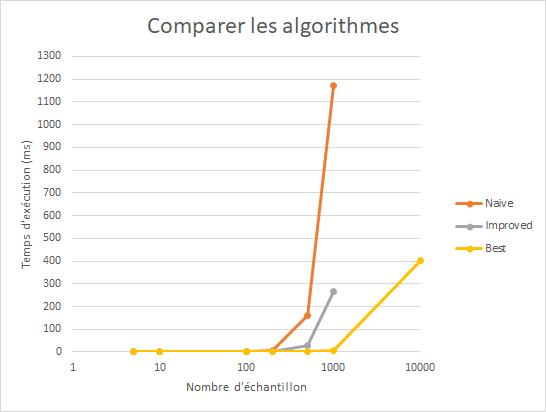
\includegraphics[width=0.8\linewidth]{img/P1_time.png}
    \caption{Graphe de temps d'exécution}
\end{figure}

\clearpage

Nous voyons clairement que l'algorithme \emph{Best} donne la solution le plus vite quand la volume des données est énorme. Nous ajoutons ici quelques visualisations de jeux données et le réseau trouvé (le code de visualiser, écrit en MATLAB, est mis dans l'annexe).

\begin{figure}[!ht]
    \centering
    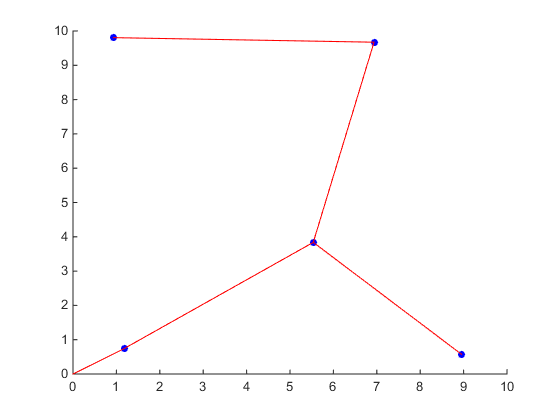
\includegraphics[width=0.8\linewidth]{img/n=5_maxX=10_maxY=10.png}
    \caption{L'arbre le plus court lorsque $N=5$}
\end{figure}

\begin{figure}[!ht]
    \centering
    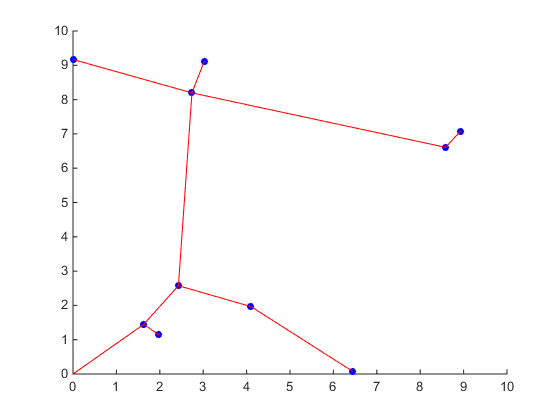
\includegraphics[width=0.8\linewidth]{img/n=10_maxX=10_maxY=10.png}
    \caption{L'arbre le plus court lorsque $N=10$}
\end{figure}

\begin{figure}[!ht]
    \centering
    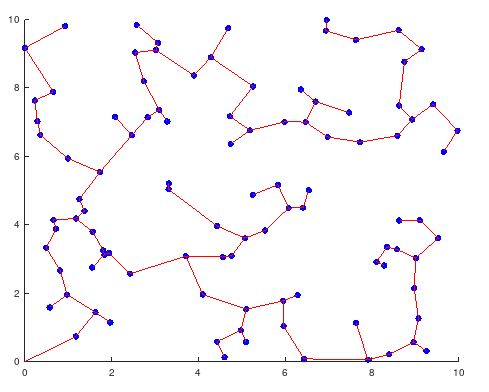
\includegraphics[width=0.8\linewidth]{img/n=100_maxX=10_maxY=10.png}
    \caption{L'arbre le plus court lorsque $N=100$}
\end{figure}

\section{Plannification de production d'huiles}

\subsection{Modèle 1}
Soient les paramètres:
\begin{itemize}
    \item $V$: l'ensemble d'huiles végétales brutes.
    \item $H$: l'ensemble d'huiles hydrogénées brutes.
    \item $B = V \cup H$: l'ensemble d'huiles brutes.
    \item $N$: le nombre de mois à plannifier.
    \item $p_f$: prix vendu de produit final. (euro/t)
    \item $p_{i,j}$: cout d'achat de l'huile $i$ au mois $j$. (euro/t)
    \item $V_{max}$: quantité maximale de raffinage d'huiles végétales. (t)
    \item $H_{max}$: quantité maximale de raffinage d'huiles hydrogénées. (t)
    \item $SM_i$: stock maximale chaque mois de l'huile $i$. (t)
    \item $c_s$: cout de stockage. (euro/t)
    \item $SI_i$: stock initial de l'huile $i$. (t)
    \item $SF_i$: stock final de l'huile $i$. (t)
    \item $v_i$: coefficient de viscosité de l'huile $i$.
    \item $v_{min}$: viscosité minimale de produit final.
    \item $v_{max}$: viscosité maximale de produit final.
\end{itemize}

Soient les variables:
\begin{itemize}
    \item $a_{i,j}$: quantité d'achat de l'huile $i$ au mois $j$. (t)
    \item $s_{i,j}$: stock de l'huile $i$ au mois $j$. (t)
    \item $r_{i,j}$: quantité de raffinage de l'huile $i$ au mois $j$. (t)
\end{itemize}

Soit $P$ le profit de l'entreprise après $N$ mois.

Le système d'équations linéaires est décrit de manière suivant:
\begin{align*}
    & \text{Maximizer } P = \sum\limits_{j = 1}^N {\sum\limits_{i \in B}^{} {{r_{i,j}}p_f} }  - \sum\limits_{j = 1}^N {\sum\limits_{i \in B}^{} {{a_{i,j}}{p_{i,j}}} }  - {c_s}\sum\limits_{j = 1}^N {\sum\limits_{i \in B}^{} {{s_{i,j}}} }\\
    & \text{Sachant que : }\\
    & \forall j = \overline {1,N} :\sum\limits_{i \in V}^{} {{r_{i,j}}}  \le {V_{\max }}\\
    & \forall j = \overline {1,N} :\sum\limits_{i \in H}^{} {{r_{i,j}}}  \le {H_{\max }}\\
    & \forall j = \overline {1,N} :\sum\limits_{i \in B}^{} {{r_{i,j}}{v_i}}  \le {v_{\max }}\sum\limits_{i \in B}^{} {{r_{i,j}}} \\
    & \forall j = \overline {1,N} :\sum\limits_{i \in B}^{} {{r_{i,j}}{v_i}}  \ge {v_{\min }}\sum\limits_{i \in B}^{} {{r_{i,j}}} \\
    & \forall j = \overline {1,N} ,\forall i \in B:{s_{i,j}} = {s_{i,j - 1}} + {a_{i,j}} - {r_{i,j}}\\
    & \forall i \in B:{s_{i,0}} = S{I_i}\\
    & \forall i \in B:{s_{i,N}} = S{F_i}\\
    & \forall j = \overline {0,N} ,\forall i \in B:S{M_i} \ge {s_{i,j}} \ge 0;{a_{i,j}} \ge 0;{r_{i,j}} \ge 0
\end{align*}

La solution sera:
\begin{itemize}
    \item Le profit maximale après $N$ mois: $P$ (euros).
    \item Au mois $j$:
    \begin{itemize}
        \item Pour l'huile $i$:
        \begin{itemize}
            \item Achater : $a_{i,j}$ tonne(s).
            \item Raffiner : $r_{i,j}$ tonne(s).
            \item Stocker : $s_{i,j}$ tonne(s).
        \end{itemize}
    \end{itemize}
\end{itemize}

\subsection{Modèle 2}
Soient les paramètres:
\begin{itemize}
    \item $V$: l'ensemble d'huiles végétales brutes.
    \item $H$: l'ensemble d'huiles hydrogénées brutes.
    \item $B = V \cup H$: l'ensemble d'huiles brutes.
    \item $N$: le nombre de mois à plannifier.
    \item $p_f$: prix vendu de produit final. (euro/t)
    \item $p_{i,j}$: cout d'achat de l'huile $i$ au mois $j$. (euro/t)
    \item $V_{max}$: quantité maximale de raffinage d'huiles végétales. (t)
    \item $H_{max}$: quantité maximale de raffinage d'huiles hydrogénées. (t)
    \item $SM_i$: stock maximale chaque mois de l'huile $i$. (t)
    \item $c_s$: cout de stockage. (euro/t)
    \item $SI_i$: stock initial de l'huile $i$. (t)
    \item $SF_i$: stock final de l'huile $i$. (t)
    \item $v_i$: coefficient de viscosité de l'huile $i$.
    \item $v_{min}$: viscosité minimale de produit final.
    \item $v_{max}$: viscosité maximale de produit final.
    \item $D = B \times B$: couples de dépendances. $(x, y) \in D$ signifie que si $x$ est utilisée, $y$ doit être utilisée aussi.
    \item $n_{max}$: nombre maximal d'huiles utilisées dans un mois.
    \item $u_{min}$: la quantité minimale si une huile est utilisée. (t)
    \item $M = V_{max} + H_{max}$: un grand nombre.
\end{itemize}

Soient les variables:
\begin{itemize}
    \item $a_{i,j}$: quantité d'achat de l'huile $i$ au mois $j$. (t)
    \item $s_{i,j}$: stock de l'huile $i$ au mois $j$. (t)
    \item $r_{i,j}$: quantité de raffinage de l'huile $i$ au mois $j$. (t)
    \item $u_{i,j}$: variable binaire, indiquant l'usage de l'huile $i$ au mois $j$.
\end{itemize}

Soit $P$ le profit de l'entreprise après $N$ mois.

Le système d'équations linéaires est décrit de manière suivant:
\begin{align*}
    & \text{Maximizer } P = \sum\limits_{j = 1}^N {\sum\limits_{i \in B}^{} {{r_{i,j}}p_f} }  - \sum\limits_{j = 1}^N {\sum\limits_{i \in B}^{} {{a_{i,j}}{p_{i,j}}} }  - {c_s}\sum\limits_{j = 1}^N {\sum\limits_{i \in B}^{} {{s_{i,j}}} }\\
    & \text{Sachant que : }\\
    & \forall j = \overline {1,N} :\sum\limits_{i \in V}^{} {{r_{i,j}}}  \le {V_{\max }}\\
    & \forall j = \overline {1,N} :\sum\limits_{i \in H}^{} {{r_{i,j}}}  \le {H_{\max }}\\
    & \forall j = \overline {1,N} :\sum\limits_{i \in B}^{} {{r_{i,j}}{v_i}}  \le {v_{\max }}\sum\limits_{i \in B}^{} {{r_{i,j}}} \\
    & \forall j = \overline {1,N} :\sum\limits_{i \in B}^{} {{r_{i,j}}{v_i}}  \ge {v_{\min }}\sum\limits_{i \in B}^{} {{r_{i,j}}} \\
    & \forall j = \overline {1,N} ,\forall i \in B:{s_{i,j}} = {s_{i,j - 1}} + {a_{i,j}} - {r_{i,j}}\\
    & \forall i \in B:{s_{i,0}} = {SI_i}\\
    & \forall i \in B:{s_{i,N}} = {SF_i}\\
    & \forall j = \overline {1,N} ,\forall i \in B:{u_{\min }}*{u_{i,j}} \le {r_{i,j}} \le M*{u_{i,j}}\\
    & \forall j = \overline {1,N} :\sum\limits_{i \in B}^{} {{u_{i,j}}}  \le {n_{\max }}\\
    & \forall j = \overline {1,N} ,\forall \left( {{i_1},{i_2}} \right) \in D:{u_{{i_1},j}} \le {u_{{i_2},j}}\\
    & \forall j = \overline {0,N} ,\forall i \in B:S{M_i} \ge {s_{i,j}} \ge 0;{a_{i,j}} \ge 0;{r_{i,j}} \ge 0
\end{align*}

La solution sera:
\begin{itemize}
    \item Le profit maximale après $N$ mois: $P$ (euros).
    \item Au mois $j$:
    \begin{itemize}
        \item Pour l'huile $i$ (si utilisée):
        \begin{itemize}
            \item Achater : $a_{i,j}$ tonne(s).
            \item Raffiner : $r_{i,j}$ tonne(s).
            \item Stocker : $s_{i,j}$ tonne(s).
        \end{itemize}
    \end{itemize}
\end{itemize}

\section{Annexe}

\end{document}